\documentclass[11pt]{beamer} %handout,
%\usepackage{pgfpages}
%\pgfpagesuselayout{2 on 1}[landscape,a4paper,border shrink=2mm]
\usetheme{Montpellier} 
\usecolortheme{rose}
\usepackage{color, colortbl}
\definecolor{ForestGreen}{RGB}{0,150,100}

\usepackage{cmap}
\usepackage[T2A]{fontenc}	
\usepackage[utf8]{inputenc}	
\usepackage[english,russian]{babel}

\setbeamercovered{transparent}
\setbeamertemplate{navigation symbols}{} % hide navigation symbols
\setbeamertemplate{footline}[frame number]

\usepackage{ulem} % enables \sout{text}
\usepackage{hyperref}

\usepackage{url}
\usepackage{pgfplots}
\pgfplotsset{compat=1.7}

\usepackage[absolute,overlay]{textpos}  % import this to allow the textblock
\usepackage{graphicx}
\graphicspath{{figures/}}
\usepackage{pgfplots}
\usepackage{pgfplotstable}

\setbeamertemplate{caption}{\raggedright\insertcaption\par}

\usepackage{array,tabularx,tabulary,booktabs}
\setbeamerfont{title}{size=\Large\normalfont}
\setbeamerfont{subtitle}{size=\normalsize\normalfont\slshape}
\setbeamerfont{author}{size=\normalsize}
\setbeamerfont{institute}{size=\normalsize\itshape}


\author{Maria Kunilovskaya}
\title[Translationese indicators for human translation quality estimation]{Translationese indicators \\for human translation quality estimation}

\subtitle{(based on English-to-Russian translation of mass-media texts)}
\institute{University of Wolverhampton}
\date{13 March, 2023}

\begin{document}
	\begin{frame}[plain]

		
\includegraphics[width=50mm]{rgcl_logo}%

		\maketitle % Титульный слайд
	\end{frame}
	
\section{Overview of research design}

\begin{frame}{General description}
	\begin{exampleblock}{`Shining-through' example}
		\hspace{5em} -- How much time? \\
		\hspace{5em} -- Five hours. \\
		\hspace{5em} -- Such much? \\
		\hspace{5em} -- For whom how ... \\
		\hspace{5em} -- Finished injaz? \\
		\hspace{5em}  -- Aaask!
	\end{exampleblock}

\begin{description}
	\item[Overarching aim:] Explore the relations between translationese indicators and human translation quality.    
	\item[Experimental setup:] Human translation quality estimation task cast as text classification or regression problems, and feature analysis.
\end{description}
\end{frame}	

\begin{frame}[plain]{Research subcorpora}
	\vspace{0.3em}
	\begin{textblock*}{2cm}(11cm, 0.2cm) % {block width} (coords)
		\includegraphics[width=1.5cm]{rusltc.jpg}
	\end{textblock*}
	\begin{enumerate}
		\item subsets from \textit{Russian Learner Translator corpus} \\of various sizes by type of annotation
		\begin{figure}
			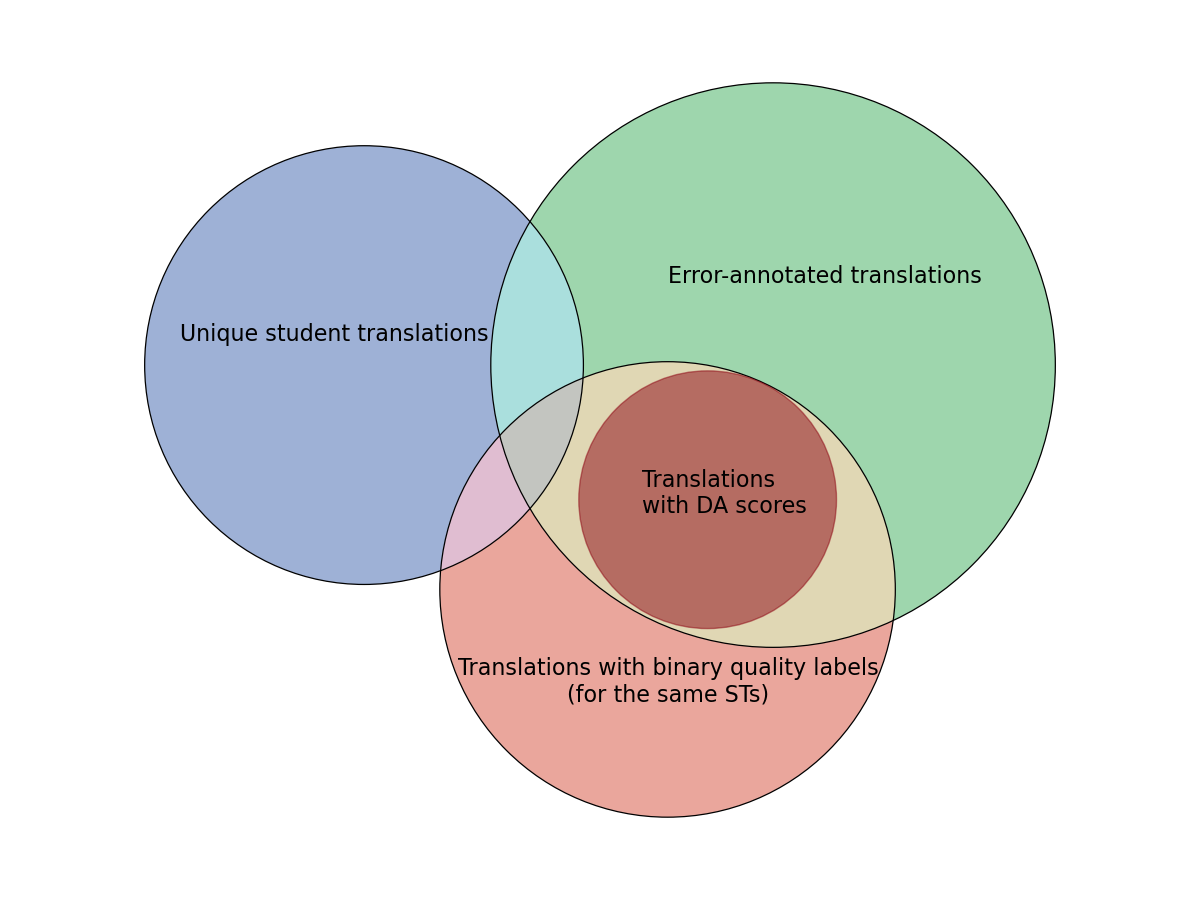
\includegraphics[width=70mm]{subsets}
		\end{figure}
		\item comparable professional translations: 404 parallel docs, 384 K words (BBC Russian Service, InoSMi, RNC);
		\item comparable non-translations: 497 docs, 523 K words (RNC)
	\end{enumerate}
	
\end{frame}

\begin{frame}{Quality labels/scores}

	Operational definitions of quality
	\begin{itemize}
		\item \textit{Holistic judgments}: agreed assessment of competition jury/exam board in real life; top and bottom grades converted to `bad', `good' labels, verified in an additional annotation experiment ($\alpha=0.524$, accuracy 91\%).
		\item Scores from \textit{error annotation} used as part of feedback to students in a real-life practical translation course, which implemented accuracy-fluency distinction (top-level category agreement: 80.5\% of errors in the same location, $\alpha=0.535$).
		\item \textit{Direct assessment}: perceived quality for sentences presented in the context on a 100-point scale (documents: $\alpha=0.541$, sentences: $\alpha=0.463$)
	\end{itemize} 
+ Known \textit{status} of translations produced by defined subjects (students, professionals).	
\end{frame}

\begin{frame}{Numeric representations}
	Proposed feature sets:
\begin{enumerate}
	\item linguistically-motivated 60 morphosyntactic and textual features (from UD annotation)
\end{enumerate}
Alternative representations:
\begin{itemize}
	\item surface-based TF-IDF
	\item 4 types of sentence embeddings and word embeddings
\end{itemize}
+ (for quality-related experiments) MTQE features (QuEst++ )

\end{frame}

\begin{frame}{Methodology}

	\begin{block}{Learning algorithms}
		\begin{itemize}
			\item default linear Support Vector Machine
			\item one-layer neural network for quality control
		\end{itemize}	
	\end{block}

	\begin{block}{Feature analysis}
		\begin{itemize}
			\item recursive feature elimination %(RFECV)
			\item univariate analysis (single-feature classifiers and regressors)
			\item statistical analyses
			\item PCA-based visualisations
		\end{itemize}
	\end{block}

\end{frame}


\section{Results and findings}

\subsection{translationese classification}

\begin{frame}{Translationese indicators}
\textbf{How good are the UD features to capture translationese?}
	\begin{columns}
		\column{.5\textwidth}	
		\begin{table}[H]
			\begin{tabular}{l|ll}
				\toprule
				representation    & Acc      & F1   \\
				\midrule
				UD (prof)       & 90.34 & 90.22 \\
				mdeberta3 (prof) & 98.44 & 98.36 \\
				\hline
				UD (stud)   & 89.41 & 88.96  \\
				mdeberta3 (stud) & 96.67 & 96.63 \\
				
				\bottomrule
			\end{tabular}
			\caption{\label{tab:stu-ref}Translation detection task}
		\end{table}
		\column{.5\textwidth}
				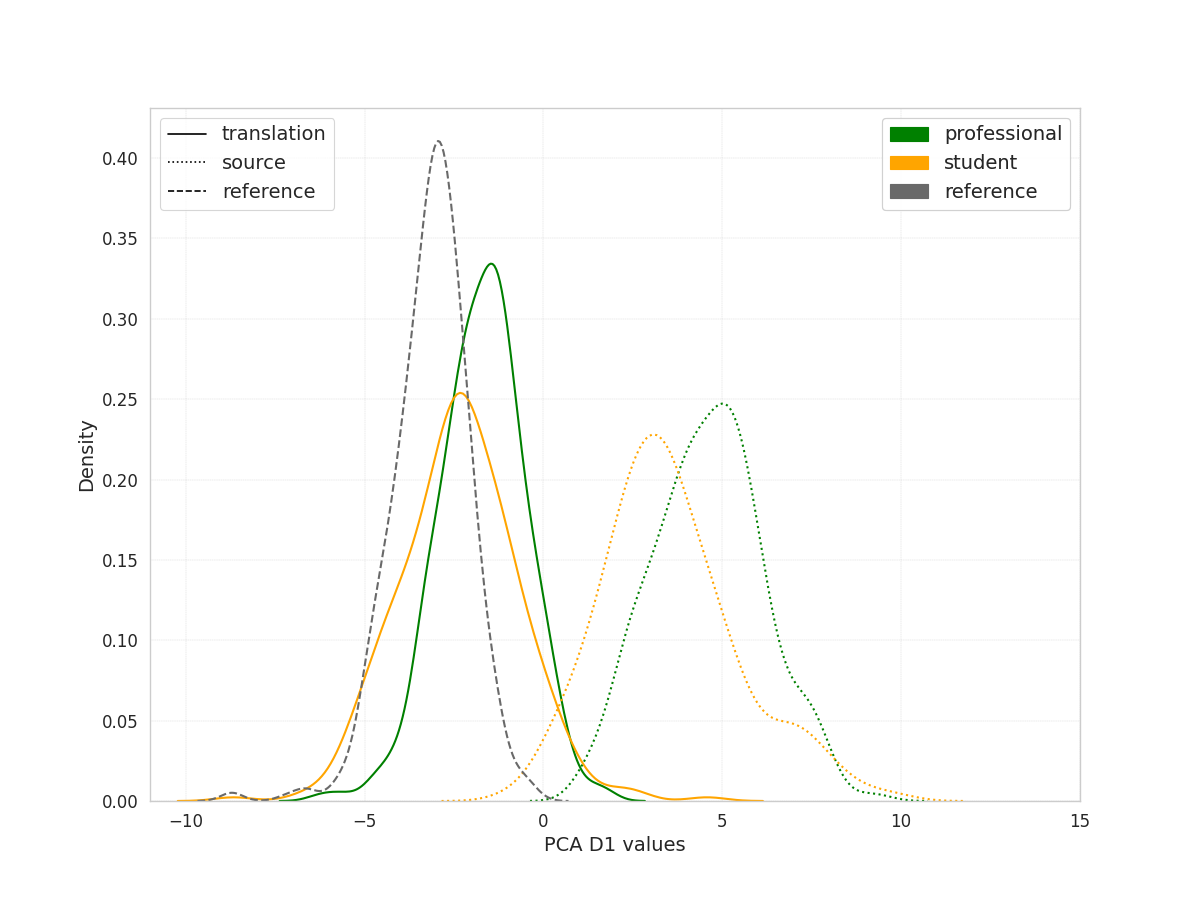
\includegraphics[width=6cm]{pca/src-var-ttype-ud-PCA-D1-lines}
		
   \end{columns}
	
\end{frame}

\begin{frame}{}
	\textbf{What are the prominent translationese indicators?}\\
	(based on feature selection)
	\begin{itemize}
		\item longer and more complex sentences
		\item inflated frequencies of \textit{additive discourse markers, analytical passives, copula verbs, modal predicates, personal pronouns, finite verbs, determiners}
	\end{itemize}
	
	\bigskip
	
	Prominent trends and associated translation strategies \\
	(based on statistical testing)
	\begin{itemize}
		\item shining through
		\item (over-)normalisation
	\end{itemize}
%	NB! dissimilarity of sources in student and professional subcorpora made analysis difficult
\end{frame}

\subsection{binary quality}

\begin{frame}{Quality estimation tasks on quality labels (linear SVM)}
	\begin{block}{professionals vs students}
		\begin{itemize}
			\item dissimilar translationese patterns (UD F1=76.24)
			\item quality related distinctions (QuEst++ F1=83.00)
			\item topical differences overshadow translationese (tf-idf F1=89.59)
		\end{itemize}
	\end{block}
	\begin{textblock*}{12cm}(9cm, 7cm) % {block width} (coords)
	{\scriptsize \textcolor{ForestGreen}{F1=68.9 on selected features}}
	\end{textblock*}
	\begin{exampleblock}{bad vs good}
		\begin{table}[H]
			\centering
			\begin{tabular}{l|ll}
				\toprule
				rep             & Accuracy & F1 \\
				\midrule
				UD              & 61.39 & 61.00 \\
				quest61         & 47.22 & 46.96 \\
				\midrule
				ruRoberta & 75.00 & 74.89 \\
				mdeberta3  & 78.33 & 78.14 \\
				\bottomrule
			\end{tabular}
		\end{table}
	
	\end{exampleblock}
\end{frame}

\begin{frame}{}
	\begin{columns}
		\column{.5\textwidth}
		UD features
		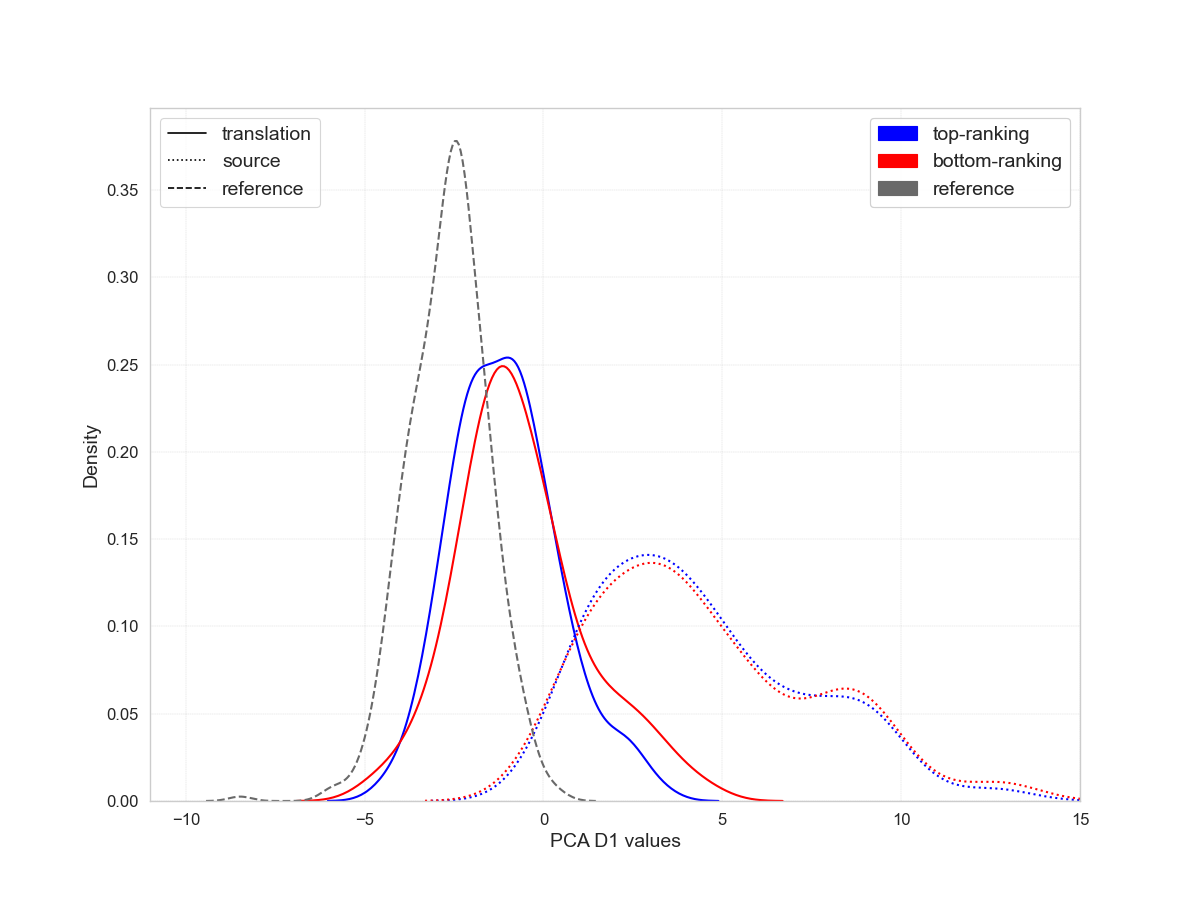
\includegraphics[width=5cm]{pca/src-qua-ttype-ud-PCA-D1-lines}
		mdeberta3 binary quality
		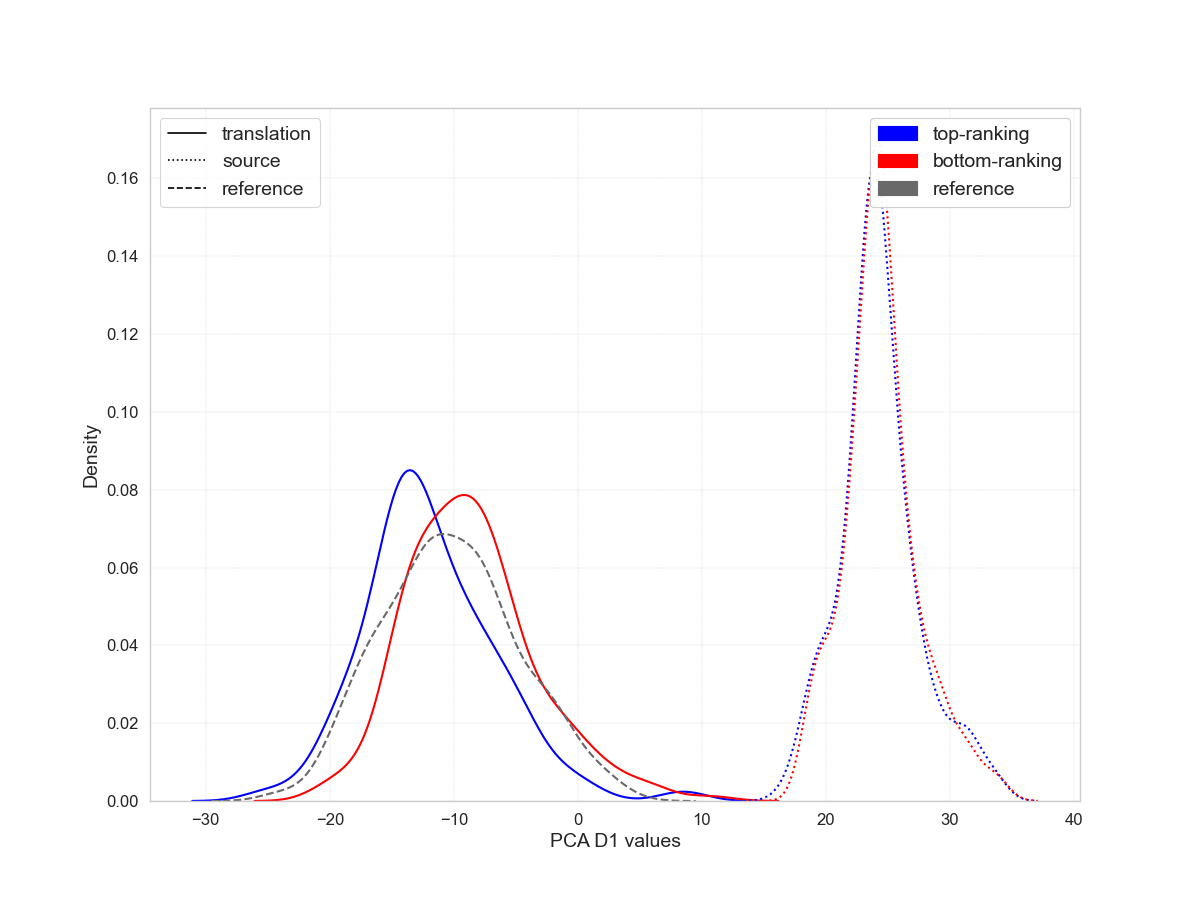
\includegraphics[width=5cm]{pca/src-qua-ttype-mdeberta3-base-PCA-D1-lines}
		\column{.5\textwidth}
		\begin{itemize}
			\item SL/TL independent translationese features are important!
			\item Bad: \footnotesize{longer sentences, complex sentence structure, lower TTR, analytical passives, more nouns as subjects, more modal predicates, more verbal (overuse of copula, deverbal nouns and participles)}
		\end{itemize}
		mdeberta3: prof experience 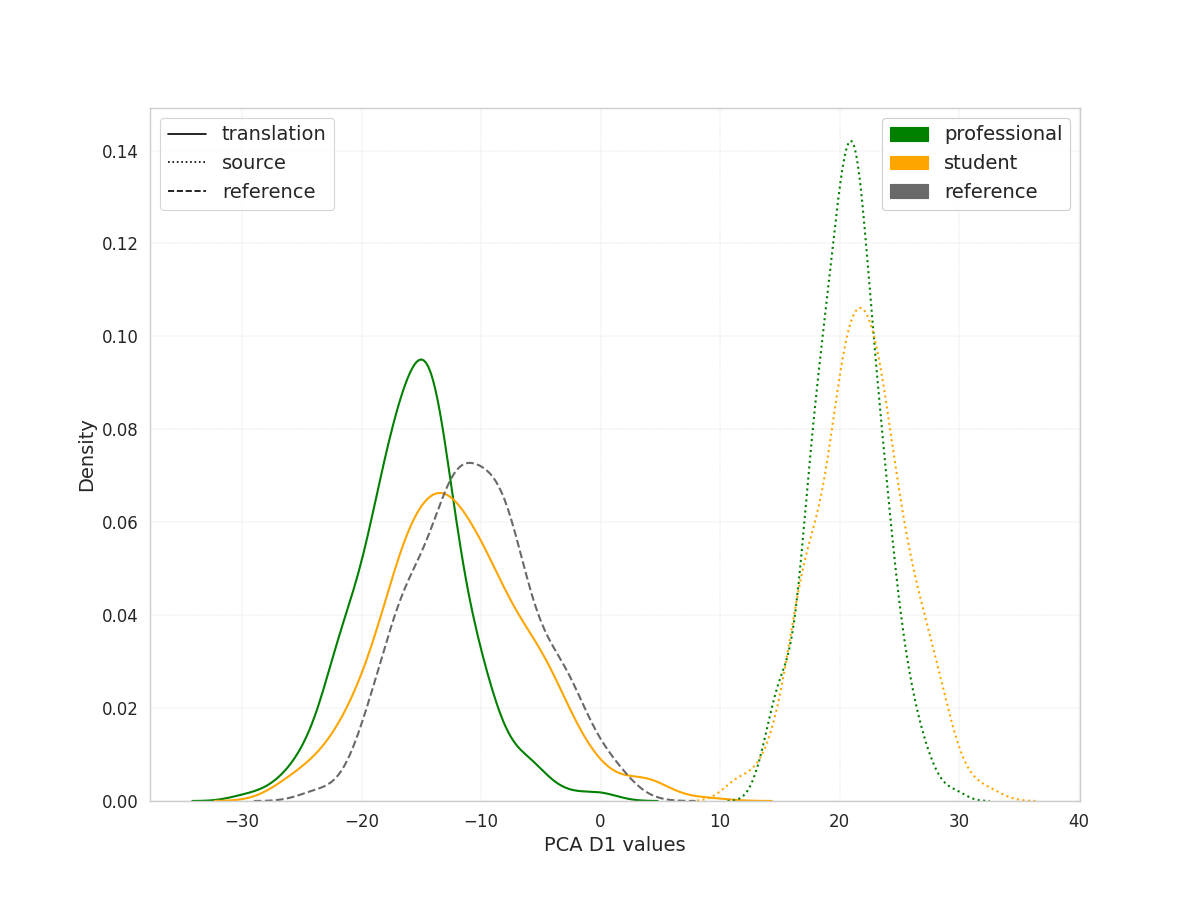
\includegraphics[width=5cm]{pca/src-var-ttype-mdeberta3-base-PCA-D1-lines.png}
	\end{columns}
\end{frame}

\subsection{continuous scores}
\begin{frame}{Scores from error annotation (553 documents)}
	
		\begin{table}[H]
		\centering
		\begin{tabular}{l|cl|cl|cl}
			\toprule
			& \multicolumn{2}{c|}{accuracy} & \multicolumn{2}{c|}{fluency}  & \multicolumn{2}{c}{tq} \\
			\midrule
			& \textit{r}  & RMSE & \textit{r}  & RMSE & \textit{r}  & RMSE\\
			\midrule
			UD     & \textbf{0.43} & 0.95 & \textbf{0.43} & 1.18 & \textbf{0.45} & 1.72\\
			quest61         & 0.37 & 0.98 & 0.42 & 1.16 & 0.36 & 1.73\\
			\midrule
			tfidf           & 0.48 & 0.92 & 0.49 & 1.14 & 0.47 & 1.69\\
			ruRoberta & 0.51 & 0.91 & 0.53 & 1.08 & 0.54 & 1.57\\
			mdeberta3  & \textbf{0.58} & 0.87 & \textbf{0.58} & 1.05 & \textbf{0.62} & 1.5\\
		\end{tabular}
		\caption{Regression results for \textit{unweighted} error-based quality scores}
	\end{table}

Observations from feature analysis: 
\begin{itemize}
	\item no difference between accuracy and fluency (!)
	\item the very weak correlations between features and scores 
	\item confusing observations for individual features
\end{itemize}
	
\end{frame}

\begin{frame}{Scores from Direct Assessment (140 documents)}
	
\begin{table}[H]
	\centering
	\begin{tabular}{l|cl}
		\toprule
		& \multicolumn{2}{c}{da\_mean} \\
		\midrule
		rep       & \textit{r}  & RMSE \\
		\midrule
		UD        & 0.23 & 7.27 \\
		quest61   & 0.18 & 7.44 \\
		\midrule
		ruRoberta & 0.22 & 7.35 \\
		mdeberta3 & 0.37 & 7.22 \\
		\bottomrule
	\end{tabular}
\end{table}
	Results:
	\begin{itemize}
		\item none of the representations was more successful than the other in learning DA scores,
		\item in fair experimental setting, \textit{mdeberta3} vectors performed better on some error-based scores than on DA scores,
		\item UD feature analysis is hardly reliable
	\end{itemize}
\end{frame}

\begin{frame}{Observations from sentence-level experiments}
	
	\begin{table}[]
		\centering
		\begin{tabular}{l|cc|c}
			\toprule
			& \multicolumn{2}{c|}{Error-based scores} & DA \\
			&  accuracy    &     fluency      & da\_mean \\
			\midrule  
			UD          & 0.17 &  0.23  & 0.29 \\
			quest70     & 0.14  & 0.25  & 0.33 \\
			\hline  
			ruRoberta    & 0.29  & 0.31 & 0.39 \\ 
			mdeberta3    & 0.27  & 0.33 & 0.39 \\ 
			\bottomrule
		\end{tabular}
		\caption{Spearman's \textit{r} on 3,224 sentence pairs (SVR)}
	\end{table}
	
	\begin{itemize}
		\item translationese-aware features were relatively competitive only for fluency scores (difference between accuracy and fluency!),
		\item an accidental finding: \\error-based quality scores reflected the properties of texts better than they fit the properties of sentences,
		\item interpretation of features does not make sense   
	\end{itemize}
\end{frame}

\section{Contributions and limitations}


\begin{frame}{Contributions}
	\begin{enumerate}
		\item a theoretically-motivated feature set for translationese diagnostics in English-to-Russian mass-media translation;
		\item evidence that lower-ranking translations exhibited more translationese than higher-ranking translations (UD features were competitive against other representations);
		\item description of dissimilar translationese patterns in professional varieties;
		\item evidence of dissimilarities between three quality assessment methods in terms of sensitivity to translationese and in terms of capturing document-level properties;
		\item datasets for document- and sentence-level HTQE experiments in English-to-Russian language pair with three types of quality judgments
	\end{enumerate}
\end{frame}

\begin{frame}{Theoretically disputable assumptions and limitations}
	\begin{enumerate}
		\item translation quality does not boil down to fluency;
		\item the approach is biased towards shining-through indicators with no distinction between negative and positive transfer;
		\item the approach is heavily-dependent on register-comparability of translations and non-translations;
		\item limited extent and reach of the study (findings apply to the given translation direction and register, given proposed features);
		\item limited application of translationese approaches to sentence-level quality estimation
	\end{enumerate}
\end{frame}

\begin{frame}[plain]
\centering
\Large \textbf{Thank you!}\\
	\vspace{.5em}
	Translationese indicators \\for human translation quality estimation\\
	\vspace{.5em}
\centering

\vspace{2em}
\small
Maria Kunilovskaya \\ 

\end{frame}

\end{document}